\section{Experimental Results and Discussion}
\label{sec:results}

All four models were trained and evaluated on the class-balanced dataset (89,832 samples; $\approx$14,972 per class) using an 80/20 stratified train-test split with a 20\% validation holdout. The test set comprised 17,967 samples.

\subsection{Overall Performance Comparison}
\label{sec:perf}

Table~\ref{tab:results} summarises the test-set performance. BiLSTM achieved the highest observed accuracy ($+1.57$\,pp over CNN, $+2.90$\,pp over SVM, $+13.77$\,pp over XGBoost). The ranking BiLSTM $>$ CNN $>$ SVM $>$ XGBoost indicates that sequential context modelling provides a measurable advantage over local feature extraction and bag-of-words approaches, with XGBoost exhibiting a substantially larger performance gap attributable to its difficulty capturing sequential dependencies in text. However, no statistical significance testing was conducted, so these differences should be interpreted cautiously.

\begin{table}[!htb]
\centering
\caption{Test-set performance comparison. All metrics are macro-averaged.}
\label{tab:results}
\footnotesize
\begin{tabular}{@{}lcccc@{}}
\toprule
\textbf{Model} & \textbf{Acc.\,(\%)} & \textbf{Prec.\,(\%)} & \textbf{Rec.\,(\%)} & \textbf{F1\,(\%)} \\
\midrule
BiLSTM   & \textbf{94.70} & \textbf{94.97} & \textbf{94.70} & \textbf{94.64} \\
CNN      & 93.13 & 93.47 & 93.13 & 93.05 \\
SVM      & 91.80 & 92.00 & 91.80 & 91.75 \\
XGBoost  & 80.93 & 85.48 & 80.93 & 81.50 \\
\bottomrule
\end{tabular}
\end{table}

\subsection{Hyperparameter Tuning}
\label{sec:hyper}

Table~\ref{tab:hyperparams} summarises the tuning strategy, search space, best configuration, and selection rationale for each model. ML models used grid search with 3-fold cross-validation; DL models used EarlyStopping (patience\,=\,3, restoring best weights) with architecture choices guided by prior work.

\begin{table*}[!htbp]
\centering
\caption{Hyperparameter search space, best configuration, and justification per model.}
\label{tab:hyperparams}
\footnotesize
\setlength{\tabcolsep}{2pt}
\resizebox{\textwidth}{!}{%
\begin{tabular}{@{}p{1.3cm}p{2.4cm}p{4.1cm}p{2.2cm}p{5.1cm}@{}}
\toprule
\textbf{Model} & \textbf{Strategy} & \textbf{Search Space} & \textbf{Best Config} & \textbf{Justification} \\
\midrule
SVM & Grid + 3-fold CV & $C \!\in\! \{0.1, 1\}$; kernel $\!\in\!$ \{lin, rbf, poly\}\textsuperscript{\dag} & $C\!=\!1$, linear & Linear kernel suits sparse TF-IDF features; $C\!=\!1$ balances margin width and misclassification~\citep{dzikovska2012using} \\
\addlinespace
XGBoost & Grid + 3-fold CV & lr $\!\in\! \{0.01, 0.1\}$; depth $\!\in\! \{5, 10\}$; est $\!\in\! \{50, 100\}$ & lr$\!=\!0.1$, depth$\!=\!10$, est$\!=\!100$ & Higher learning rate with deeper trees captures non-linear feature interactions~\citep{chen2016xgboost} \\
\addlinespace
CNN & EarlyStopping (pat.\,=\,3) & \begin{tabular}[t]{@{}l@{}}2$\times$Conv (256$\!\rightarrow\!$128, $k\!=\!5$),\\MaxPool, Dense(64), drop$\!=\!0.5{\times}2$\end{tabular} & Best ep.\,3/6 & Kernel size 5 captures bigram--trigram patterns; two Conv blocks increase receptive field~\citep{hasan2019emotion} \\
\addlinespace
BiLSTM & EarlyStopping (pat.\,=\,3) & \begin{tabular}[t]{@{}l@{}}2$\times$BiLSTM (256$\!\rightarrow\!$128),\\Dense(128$\!\rightarrow\!$64), drop$\!=\!0.5{\times}3$\end{tabular} & Best ep.\,3/6 & Stacked BiLSTM with tapering units captures hierarchical context; dropout 0.5 prevents overfitting~\citep{sun2023bidirectional} \\
\bottomrule
\end{tabular}
}
\end{table*}

The hyperparameter search was intentionally constrained to ensure controlled comparison rather than exhaustive optimisation, which may limit each model's true ceiling. For ML models, the grid targeted the most impactful parameters; for DL models, architecture choices were guided by prior work and validated through the ablation study (Section~\ref{sec:ablation}).

\subsection{Confusion Matrix and Error Analysis}
\label{sec:confusion}

\begin{figure}[!htb]
\centering
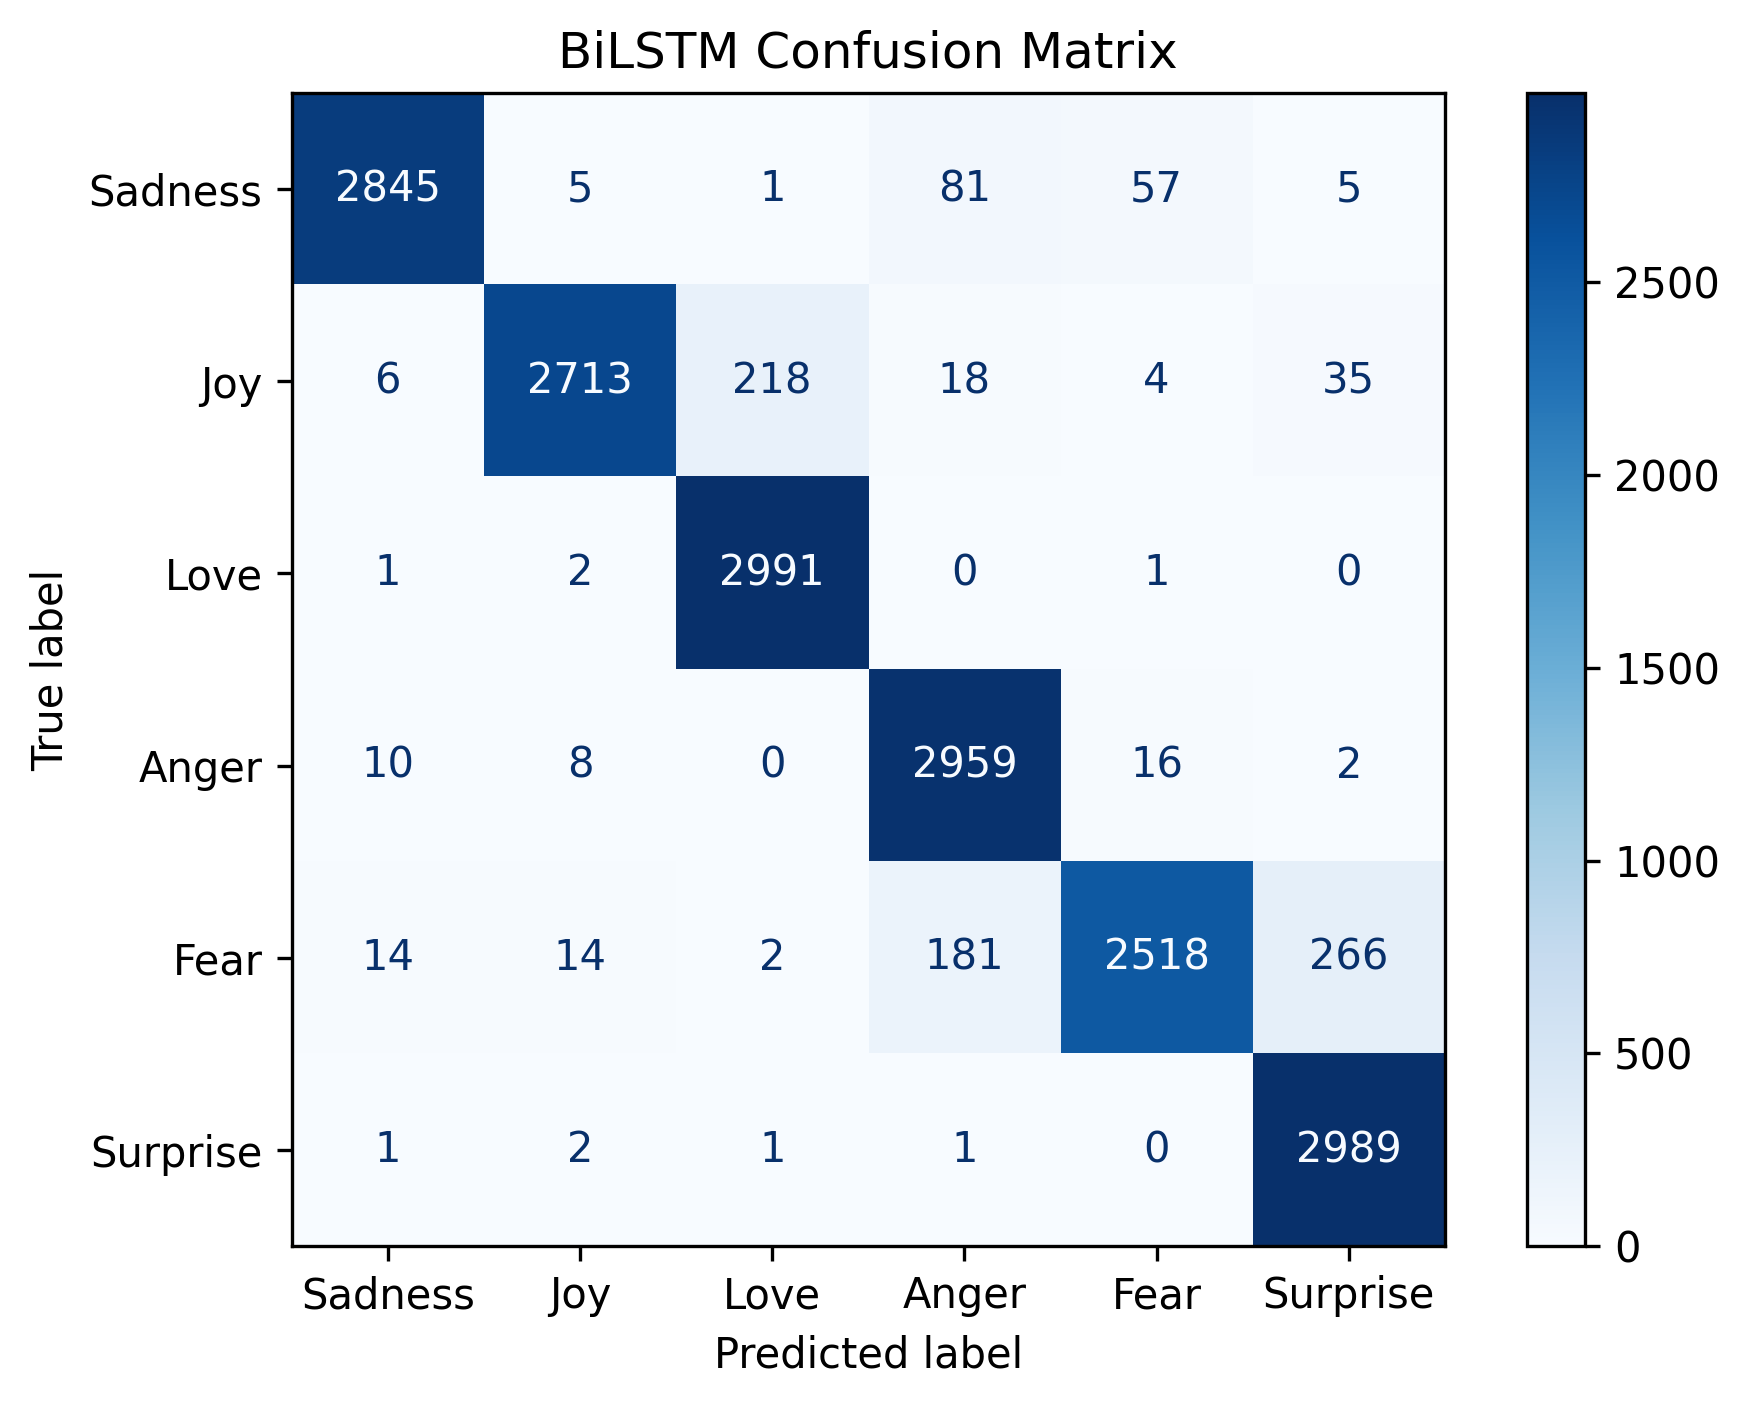
\includegraphics[width=0.75\linewidth]{figures/bilstm_confusion_matrix.png}
\vspace{-4pt}
\caption{BiLSTM confusion matrix on the test set.}
\label{fig:confusion_bilstm}
\end{figure}

Figure~\ref{fig:confusion_bilstm} presents the confusion matrix for the best-performing BiLSTM model. Three systematic error patterns persisted across all architectures (full matrices in Figure~\ref{fig:confusion_matrices}, Appendix):

\begin{enumerate}[nosep]
    \item \textbf{Valence conflation (Joy $\leftrightarrow$ Love).} All models showed notable Joy$\rightarrow$Love misclassification (see Figure~\ref{fig:confusion_matrices}), reflecting shared positively-valenced vocabulary (``happy'', ``amazing'').
    \item \textbf{Arousal ambiguity (Fear $\rightarrow$ Surprise).} Fear was frequently predicted as Surprise across all architectures (see Figure~\ref{fig:confusion_matrices}), due to shared high-arousal tokens (``shocked'', ``suddenly'') where the two emotions differ primarily in valence.
    \item \textbf{Residual majority-class bias (XGBoost).} Despite class-balanced training, XGBoost still misclassified negatively-valenced samples as Joy, with elevated Sadness$\rightarrow$Joy, Anger$\rightarrow$Joy, and Fear$\rightarrow$Joy off-diagonal counts (see Figure~\ref{fig:confusion_matrices}d).
\end{enumerate}

Per-class word clouds (Figure~\ref{fig:wordclouds} in the Appendix) corroborate these patterns. At the dataset level, four biases should be acknowledged: \textbf{platform bias} (Twitter-only corpus may not generalise to longer-form text); \textbf{annotation bias} from crowd-sourced labels~\citep{demszky2020goemotions}; \textbf{temporal bias} from evolving language; and a \textbf{label granularity constraint} (single-label taxonomy cannot capture mixed emotions).

\subsection{Training Dynamics and Computational Cost}
\label{sec:compute}

\begin{figure*}[!htbp]
\centering
\begin{minipage}{0.48\textwidth}
  \centering
  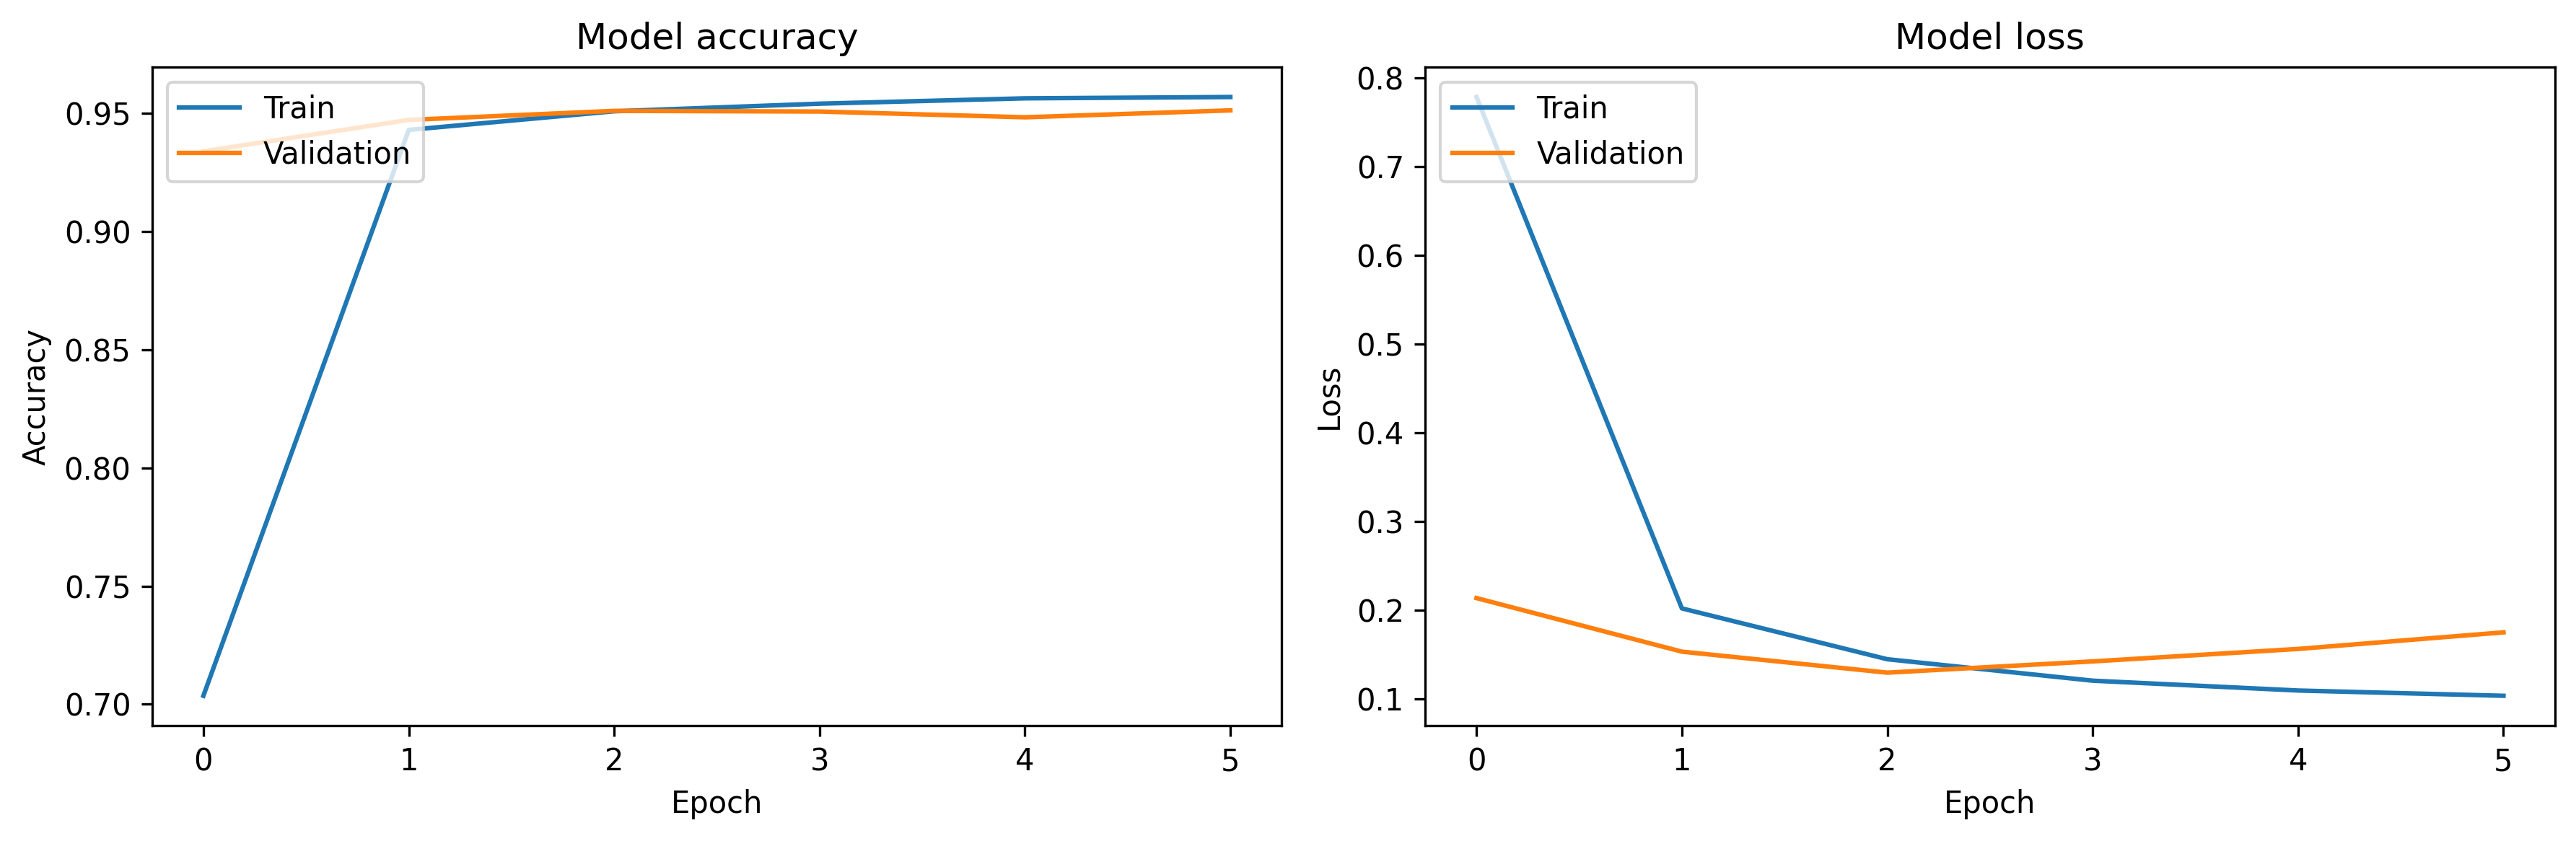
\includegraphics[width=\linewidth]{figures/bilstm_training_curves.png}
  \captionof{figure}{BiLSTM training curves (trained for 10 epochs with EarlyStopping, stopped at epoch~6). Convergence at epoch~3 with minimal train--val gap ($\approx$0.5\,pp).}
  \label{fig:train_bilstm}
\end{minipage}\hfill
\begin{minipage}{0.48\textwidth}
  \centering
  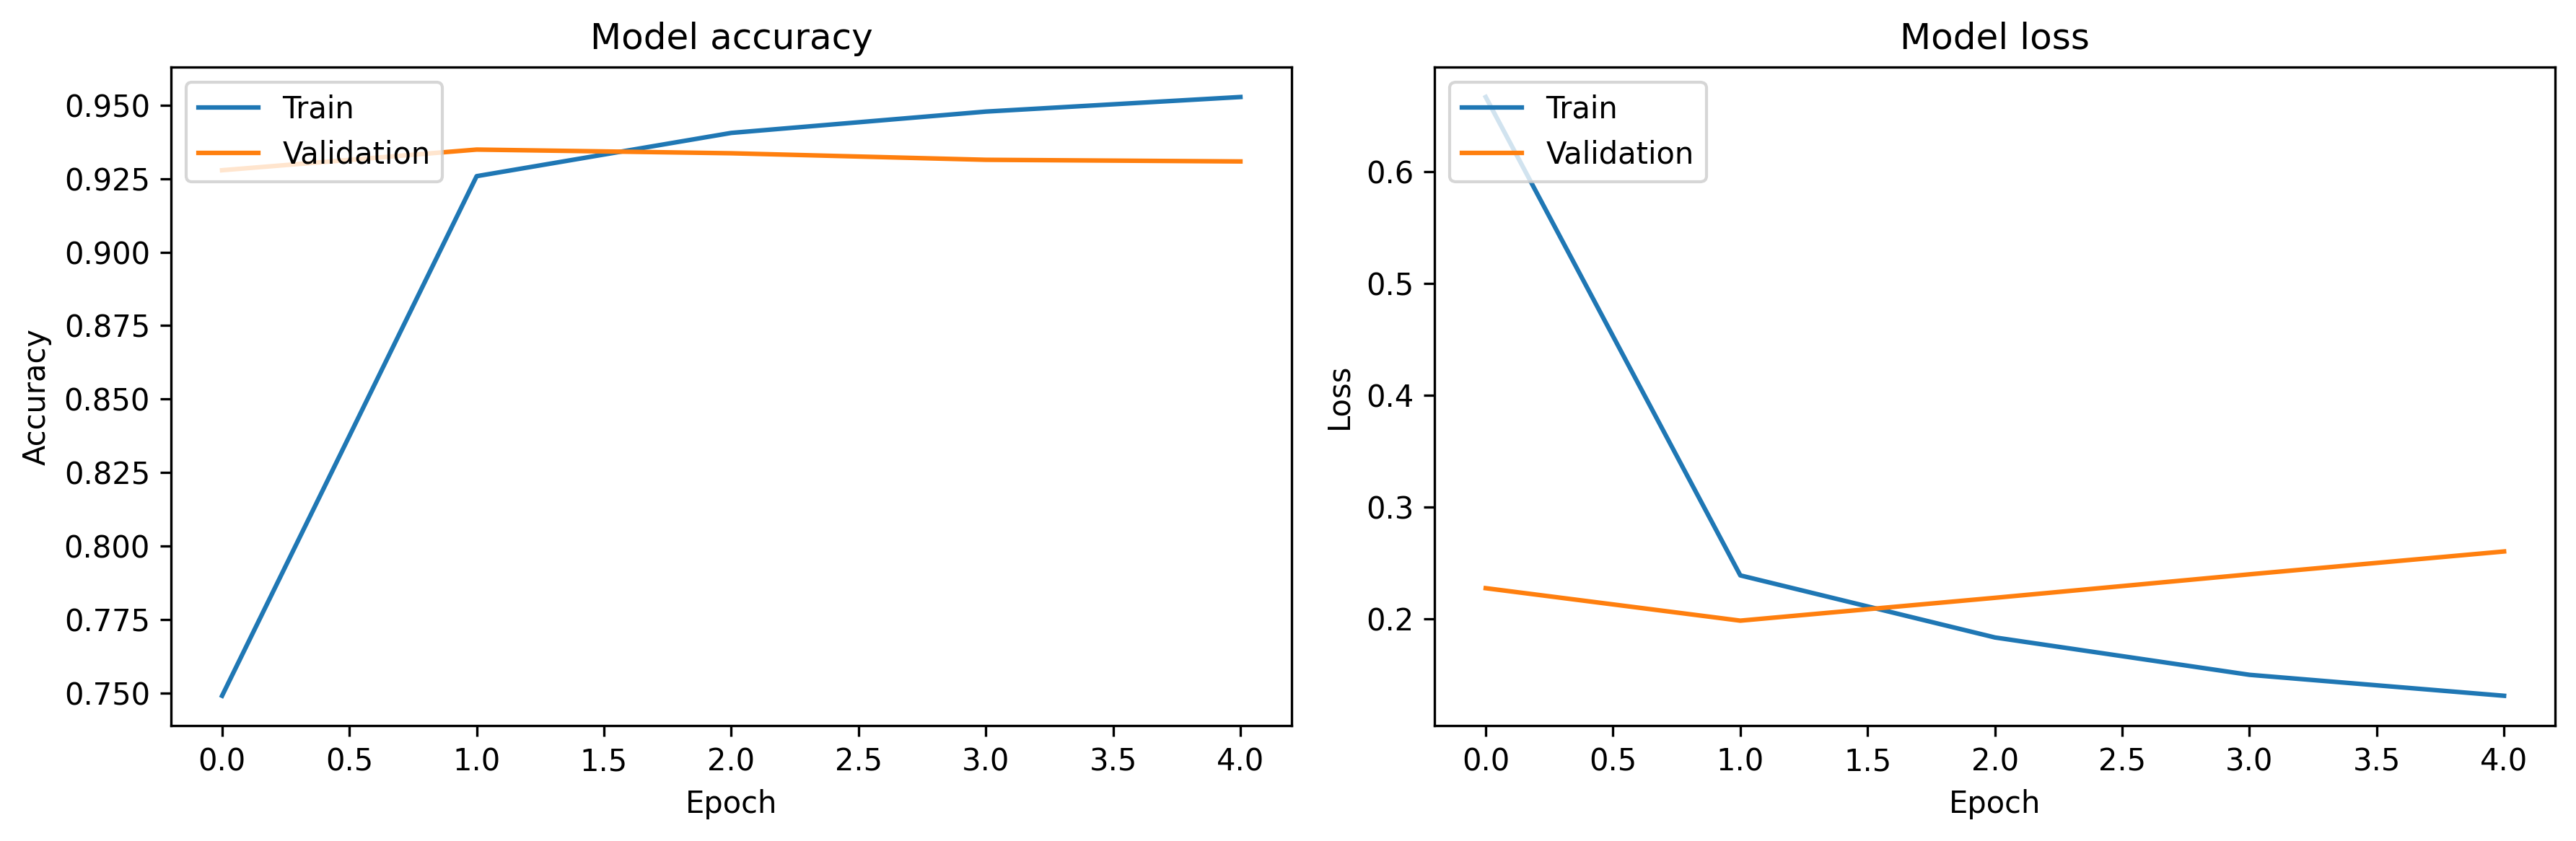
\includegraphics[width=\linewidth]{figures/cnn_training_curves.png}
  \captionof{figure}{CNN training curves (trained for 10 epochs with EarlyStopping, stopped at epoch~6). Early overfitting signs appear after epoch~3.}
  \label{fig:train_cnn}
\end{minipage}
\end{figure*}

Figure~\ref{fig:train_bilstm} shows BiLSTM converged by epoch~3 (94.17\% validation accuracy) with a small train-val gap (${\approx}0.5$\,pp), confirming good generalisation. Figure~\ref{fig:train_cnn} shows CNN reaching 92.77\% validation accuracy at epoch~3 with early signs of overfitting.

Table~\ref{tab:compute} reports computational cost. SVM required the least training time while delivering the second-highest accuracy, making it the most efficient on a performance-per-compute basis. BiLSTM demanded $12\times$ the training time of SVM for a 2.90\,pp accuracy gain and ${\sim}23\times$ higher inference latency, motivating SVM's selection for deployment.

\begin{table}[!htb]
\centering
\caption{Computational cost comparison across models.}
\label{tab:compute}
\footnotesize
\begin{tabular}{@{}lccc@{}}
\toprule
\textbf{Model} & \textbf{Train Time} & \textbf{Inference} & \textbf{Model Size} \\
\midrule
SVM      & $\sim$2\,min  & $<$1\,ms/sample  & 10\,MB \\
XGBoost  & $\sim$8\,min  & $<$1\,ms/sample  & 12\,MB \\
CNN      & $\sim$2\,min (6 ep.) & $\sim$3\,ms/sample & 4.2\,MB \\
BiLSTM   & $\sim$24\,min (6 ep.) & $\sim$23\,ms/sample & 5.6\,MB \\
\bottomrule
\end{tabular}
\end{table}

\subsection{Discussion}
\label{sec:discussion}

The high performance of the three best models (91.80--94.70\% accuracy) can be attributed to three factors:
(1)~\textbf{effective class balancing} --- downsampling to 14,972 samples per class eliminated the 9.5:1 imbalance ratio, with macro-F1 closely tracking accuracy for SVM, CNN, and BiLSTM ($\leq$0.08\,pp gap);
(2)~\textbf{the preprocessing pipeline} --- the ablation study (Section~\ref{sec:ablation}) showed the full eight-step pipeline contributes $1.42$\,pp over raw text, notably by retaining negation words that preserve discriminative signals (``not happy'' vs.\ ``happy''); and
(3)~\textbf{dataset characteristics} --- the corpus comprises short, emotionally explicit tweets (median 86 characters) with direct lexical cues, favouring both TF-IDF and embedding-based models. The 2.90\,pp gap between SVM and BiLSTM reflects the added value of sequential context modelling for order-dependent cases (\eg, ``I am not afraid'' vs.\ ``I am afraid''). XGBoost's substantially lower accuracy (80.93\%) suggests that gradient-boosted trees over TF-IDF features struggle to capture the sequential and compositional patterns critical for fine-grained emotion discrimination.

The performance ceiling appears to be bounded by \textbf{inherent label ambiguity}: the architecture-independent Joy$\leftrightarrow$Love and Fear$\rightarrow$Surprise confusion patterns (Section~\ref{sec:confusion}) persist regardless of model complexity, indicating that the remaining ${\sim}5\%$ error rate (for the best model) reflects genuine semantic overlap rather than model inadequacy~\citep{demszky2020goemotions}. Further gains may require richer representations (\eg, transformer-based contextual embeddings) rather than architectural scaling within the current feature space.

\subsection{Interpretability and Deployment Feasibility}
\label{sec:deploy}

SVM offered the highest interpretability through its linear weight vector~$w$; XGBoost provided moderate interpretability via feature importance scores; CNN and BiLSTM remained black-box models. Figure~\ref{fig:joy_demo} shows a sample prediction classified as Joy with 95.9\% confidence alongside the full preprocessing trace (additional screenshots in Appendix~\ref{sec:app_ui}). Table~\ref{tab:feasibility} summarises the deployment assessment: SVM achieved the best balance of latency, interpretability, and accuracy.

\begin{table}[H]
\centering
\caption{Deployment feasibility assessment across models.}
\label{tab:feasibility}
\footnotesize
\setlength{\tabcolsep}{3pt}
\begin{tabular}{@{}lcccc@{}}
\toprule
\textbf{Criterion} & \textbf{SVM} & \textbf{XGB} & \textbf{CNN} & \textbf{BiLSTM} \\
\midrule
Inference latency  & \cmark & \cmark & $\sim$ & \xmark \\
Memory footprint   & $\sim$ & \cmark & \cmark & \cmark \\
Interpretability   & \cmark & $\sim$ & \xmark & \xmark \\
Accuracy           & $\sim$ & \xmark & $\sim$ & \cmark \\
\bottomrule
\end{tabular}
\end{table}

\begin{figure}[H]
\centering
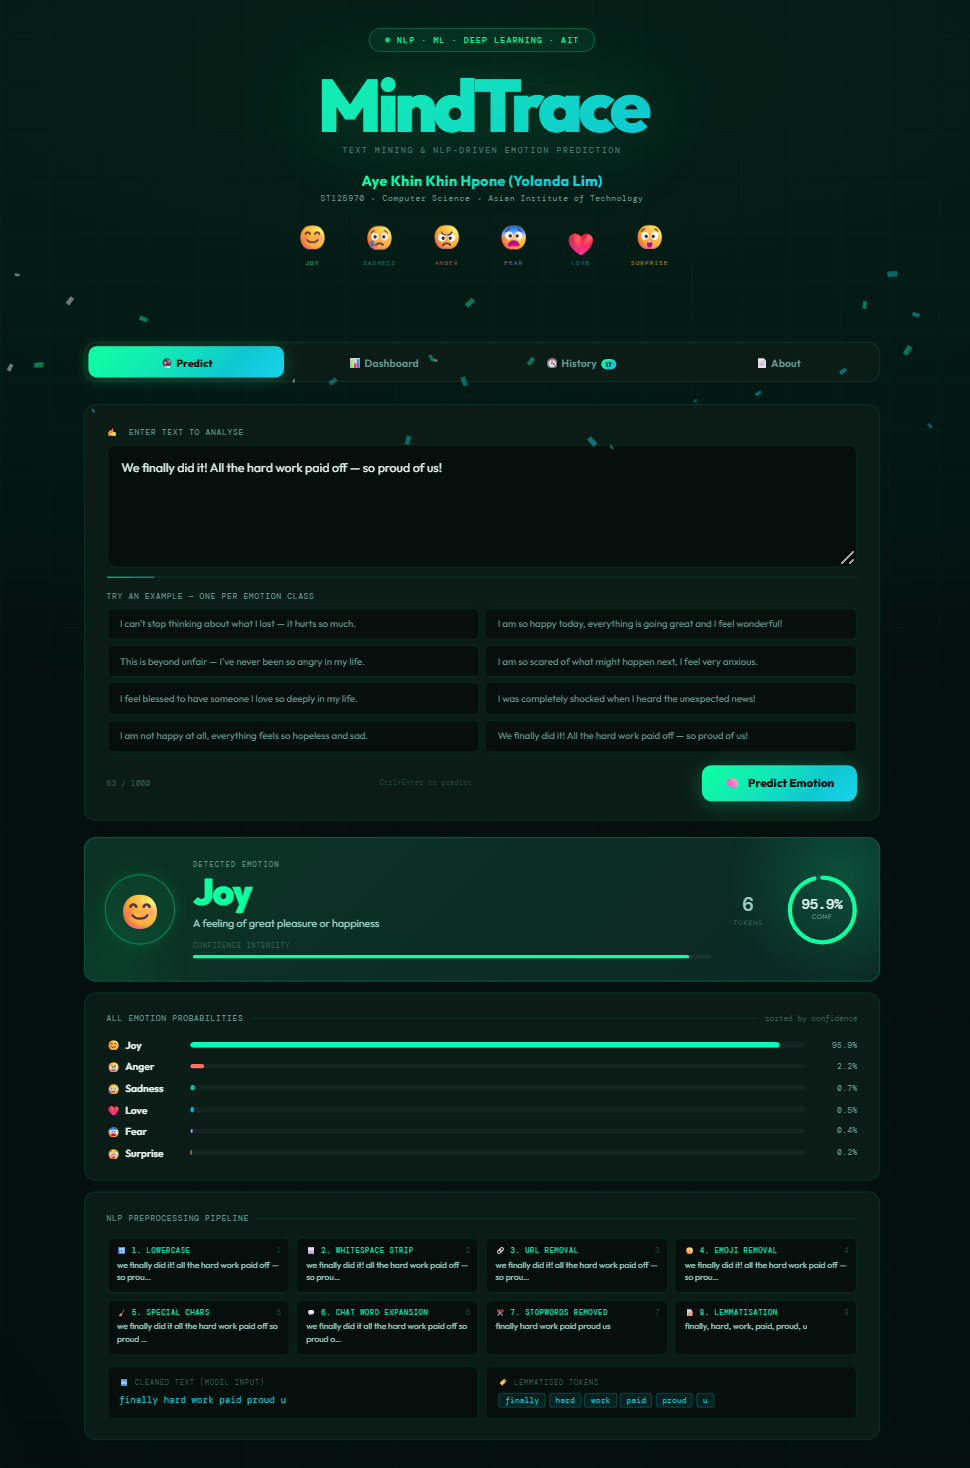
\includegraphics[width=0.85\linewidth]{img/joy.png}
\caption{MindTrace web application --- sample prediction for the Joy emotion class (95.9\% confidence). The interface displays per-class probability scores and the complete NLP preprocessing pipeline trace.}
\label{fig:joy_demo}
\end{figure}
